%========================%
%        Preamble        %
%========================%
\documentclass[12pt]{amsart}

    %========================%
%        Packages        %
%========================%

\usepackage[utf8]{inputenc}
%\usepackage{amsmath}    % Included in amsart package
%\usepackage{amsthm}     % 
\usepackage{amssymb}      % 
\usepackage{mathtools}      % Paired Limiter Macros
% \usepackage{mdframed}       % boxes for theorem
\usepackage{enumitem}     % Continuous numbering of lists
\usepackage[hidelinks]{hyperref}
\usepackage{tikz}
\usetikzlibrary{positioning}
\usepackage{blindtext}
\usepackage{graphicx}
\usepackage{float}

%========================% 
%          Title         %
%========================% 
\title{Lecture 3 and 4}
\author{Anish Sundaram}
\date{\today}

%========================% 
%        Theorems        %
%========================% 
\theoremstyle{definition}
\newtheorem{theorem}{Theorem}  % Boxed theorems
\newtheorem{definition}{Definition} % Definitions
\newtheorem{example}{Example}       %
\newtheorem{algorithm}{Algorithm}
\newtheorem*{proof*}{Proof}         % non-numbered
\newtheorem*{remark}{Remark}        %
\numberwithin{equation}{theorem}    % Local equation numbering

\setcounter{tocdepth}{3}      % Show subsubsections in contents

%========================% 
%        Macros          %
%========================% 
\DeclarePairedDelimiter\abs{\lvert}{\rvert}  % Vertical bars
\DeclarePairedDelimiter\norm{\lVert}{\rVert} % Double vertical bars
\newcommand{\drawvec}[1]{                    % matrices on one line
    \begin{bmatrix}
        #1
    \end{bmatrix}
}


% \begin{figure}[H]
%     \centering
%     \includegraphics[width=5in]{global-carbon-cycle.png}
%     \caption{The Global Carbon Cycle}
%     \label{global-carbon-cycle}
% \end{figure}

%========================% 
%         Document       %
%========================% 
\begin{document}

\maketitle

\tableofcontents

\section*{3 Probability – intuition and fundamentals}
\subsection*{3.1 Elements of Probability}

\begin{definition}
    \textbf{Experiment}:
    A situation under which a specific treatment is applied to a group and one group is left untreated as a control group in order to compare effectiveness vs placebo. This is the basis of forming conclusions
\end{definition}

\begin{definition}
    \textbf{Probability($P$)}:
    The likelyhood of an event to occur, represented as a proportion of the times an event occurs over the total amount of events. Represented as 
    $$p_n = \frac{\text{times A occurs}}{n} \longrightarrow P(A)$$ with n approaching infinity
\end{definition}

\begin{definition}
    \textbf{Sample Space($\Omega/S/U$)}:
    The total number of possible solutions to a roll, pull, Probabilistic event. it is the superset of all possible results.
\end{definition}


\begin{definition}
    \textbf{Events}:
    An statistic event is defined as an outcome or defined collection of outcomes of a random experiment. Every Event A is a subset of the Sample Space in that : $$A \subset \Omega$$
\end{definition}

\begin{figure}[H]
    \centering
    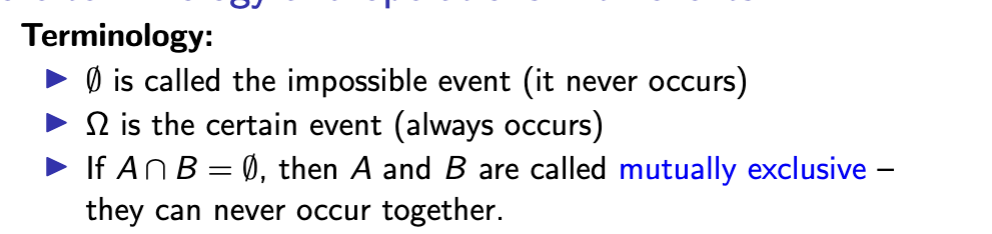
\includegraphics[width=3in]{Media/terminology.png}
    \caption{Additional terminology of sets}
    \label{terminology}
\end{figure}


\subsection*{3.2 Operations with Events}

\begin{definition}
    \textbf{Operations with Events}:
    \begin{enumerate}
        \item \textbf{Intersection($\cap$)}:
            The elementary outcomes that are in BOTH A and B: $AB = A \cap B={\omega \in \Omega  :\omega \in A \text{AND} \omega \in B}$
        \item \textbf{Union($\cup$)}:
            The elementary outcomes that are in either A,B, or both inclusive: $AB = A \cup B={\omega \in \Omega  :\omega \in A \text{OR} \omega \in B}$
        \item \textbf{Complement($A^c$)}:
            The elementary outcomes that are not in A: $A_c = {\omega \in \Omega : \omega \notin A}$
        \item \textbf{Symmetric Difference($A\Delta B$)}:
            The elementary outcomes that are in A or B BUT NOT IN BOTH: $A\Delta B = A_c B \cup AB_c = {\omega \in \Omega : \omega \in A or \omega \in B \text{but not in both}}$ This is exclusive or "XOR" operation
    \end{enumerate} 
\end{definition}

\begin{figure}[H]
    \centering
    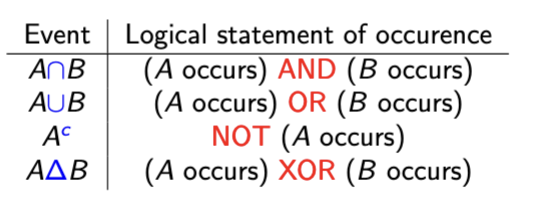
\includegraphics[width=3in]{Media/optable.png}
    \caption{Table of Set Operations}
    \label{optable}
\end{figure}

\begin{definition}
    \textbf{Set Properties}:
    There are some identities to know when dealing with sets:
    \begin{figure}[H]
        \centering
        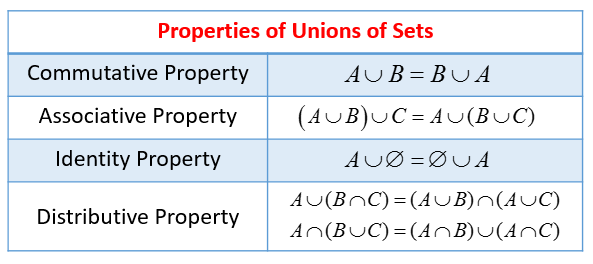
\includegraphics[width=3in]{Media/setproperties.png}
        \caption{Properties of sets}
        \label{setproperties}
    \end{figure}
\end{definition}

\subsection*{3.3 Probability}

\begin{theorem}
    \textit{Axioms of Probability}:
    The probability $P$ is required to follow the following axioms:
    \begin{enumerate}
        \item $P(\Omega) = 1$
        \item $P(A) \in [0,1],\text{for all events } A \in F$
        \item If we have a sequence of pair-wise Mutually exclusive events then: $P(U_i,A_i) = \Sigma_i P(A_i)$
    \end{enumerate}
    \begin{remark}
        The triplet $(\Omega,F,P)$ is called a \textbf{probability space}.
    \end{remark}
\end{theorem}

\begin{definition}
    \textbf{Mutually Exclusive Events}:
    2 Events that cannot happen at the same time, or in other words the intersection of set A and set B is the null set. If the probability of both is anything other than null it is \textbf{mutually inclusive}.
    $$A = [1,2,3], B = [5,6] ; A \cap B = \emptyset \text{ and } P(A \cap B) = 0$$

\end{definition}

\begin{theorem}
    \textit{Addition Rule of Probability}: A rule for breaking apart a set union which works regardess of inclusivity/exclusivity:
    $$P(A \cup B) = P(A) + P(B) - P{(A\cap B)}$$
\end{theorem}

\begin{theorem}
    \textit{Inclusion-Exclusion Principle}: States that the addition rule of probability can be extended however many times a union is applied between two sets and can continue ad infinitum: 
    $$P(A\cup B \cup C) = P(A) + P(B) + P(C) - P(A\cap B) - P(A\cap C) - P(B\cap C) - P(B\cap C) + P(A\cap B\cap C)$$
\end{theorem}

\subsection*{3.4 Fundamental Principle of Counting}

\begin{theorem}
    \textit{Fundamental Principle of Counting}:
    If there are $p$ ways to do one thing and $q$ ways to do another thing, there are $p \cdot q$ ways to do both. 
\end{theorem}

\subsection*{3.5 Permutations}
\begin{definition}
    \textbf{Permutations(P)}:
    Order of individual events does matter. Permutations are written as: $$_nP_R = \frac{n!}{(n-R)!}$$
\end{definition}

\subsection*{3.6 Combinations}

\begin{definition}
    \textbf{Combinations(C)}:
    Order of events doesnt matter. Combinations are written as:
    $$_nC_R = \frac{n!}{(n-R)!R!}$$ 
\end{definition}

\subsection*{3.7 Multinomial Coefficients}

\begin{definition}
    \textbf{Multinomial Coefficients}:
    Generalizations of binomial coefficients with a combinatorial interpretation. Because we have copies of the same letter multiple times we must discount the total number of permutations. 
     
\end{definition}

\section*{4 Conditional Probability and Independence}

\subsection*{4.1 Conditional Probability}

\begin{definition}
    \textbf{Conditional Probability}:
    The conditional probabilty of an event A given B has occured, or just A given B. This is the same as the probability of the intersection of the two events over the probability of event B:
    $$\emph{P}(A|B) = \frac{\emph{P}(A \cup B)}{\emph{P}(B)}$$
    \begin{remark}
        In a sense, because we know that B has occured it can become out new sample space and thus we re-weight the probability of A accordingly.
    \end{remark}
\end{definition}

\subsection*{4.2 Independence}

\begin{definition}
    \textbf{Independence}: Two events are said to be independent if one event's occurence does not influence the probability that the other event will or will not occur. In math terms it can be defined as :
    $$\textit(P)(AB) = \textit{P}(A)\textit{P}(B)$$
    \begin{remark}
        Logically if two events are independent then their conditional probability will equal the individual probability as the two are not linked, in other words $$P(A|B) = \frac{P(AB)}{P(B)} = \frac{P(A)P(B)}{P(B)} = P(A)$$ and the reverse will also be true in that $$P(B|A) = P(B)$$
    \end{remark}
\end{definition}

\begin{definition}
    \textbf{Independence and exclusivity}:
    If A and B are independent then so are $A^c$ and $B$ in that 
    $$P(A^cB) + P(AB) = P(B) \rightleftarrows P(A^cB) = P(B)(1-P(A)) = P(B)P(A^c)$$
    \begin{remark}
        If A and B are mutually exclusive then $P(A|B) = 0$ and so unless $P(A) = 0$, two mutually exlusive events are dependent.
    \end{remark}
\end{definition}


\subsection*{4.3 Mutually Independent Events}

\begin{definition}
    \textbf{Mutually Independence}:
    Each event is independent of any combination of other events in the collection, in other words in a collection of events there is no independence among any of them. Events are said to be mutually indepent if for all events $$P(A_1 \cup A_2 \cup \ldots A_k) = P(A_1)P(A_k)$$
\end{definition}

\subsection*{4.4 Law of total P}

\begin{theorem}
    \textit{Law of Total Probability}:
    A fundamental rule relating marginal probabilities to conditional probabilities. It expresses the total probability of an outcome which can be realized via several distinct events:
    $$P(A) = P(A|B_1) \cdot P(B_1) + P(A|B_2) \cdot P(B_2) \ldots P(A|B_x) \cdot P(B_X)$$

\end{theorem}


\subsection*{4.5 Bayes Theorem}

\begin{theorem}
    \textit{Bayes Theorem}:
    A theorem whichdescribes the probability of an event, based on prior knowledge of conditions that might be related to the event:
    $$P(A|B) = \frac{P(B|A)P(A)}{P(B)}$$

\end{theorem}

\end{document}